or for matrix form after simplification:
$$
	\beta = \left ( X^T X \right )^{-1} X^T Y
$$

In case, when matrix $X^T X$ is ill-conditioned, the solution may be not qualitative. To avoid unstably solution, regularization term $\lambda \beta^T \beta$  adds to \eqref{eq:linear_matrix_form}:
\begin{equation}
	Y = X \beta + \lambda \beta^T \beta \implies \beta = \left ( X^T X + \lambda I \right )^{-1} X^T Y, \quad \lambda \in R
\end{equation}
with this regularization term the matrix - $X^T X + \lambda I$ is better conditioned, for more details \cite{kress2012numerical} % [corollary 5.8, relation 5.22]


More advanced regression models include regularization term to the loss function, for example, Ridge regression and Lasso regression. More details are well explained in \cite{ridge}, \cite{lasso}, \cite{dantzig_selector}, \cite{rlad}, \cite{slope}

\begin{figure}[h]
	\centering
	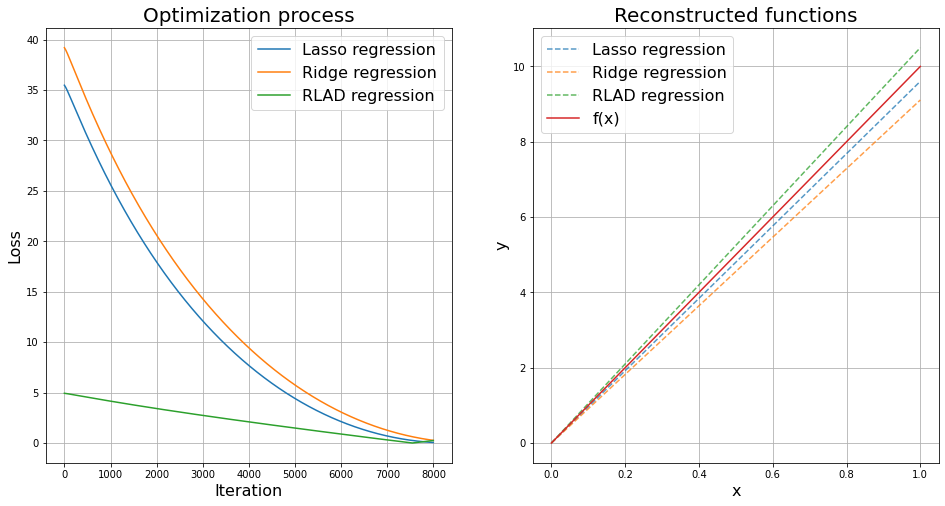
\includegraphics[width=0.8 \textwidth]{images/chapter2/reularization_impact.png}
	\caption{Comparison of different regularizations}
	\label{fig:regularizations}
\end{figure}

\paragraph{Example 1}
Let $y = f(x) = k  x + \epsilon, k = 10$. At the fig. \ref{fig:regularizations} seen, that regularization impact is big. After applying linear models for this problem with different regularization methods was got a different results. It is an important fact for the next work, where more complex regression models will be used. 

\subsection{Another methods for approximation}

There are other methods for function approximation, more specific: series expansion (Taylor series), polynomials approximation, expansion to orthogonal series(Fourier series, for example), moreover, modern approaches Randon Forest, Gradient Boosting \cite{bishop} machines or the most powerful - Neural Networks \cite{haykin}.

\paragraph{Example 2}
Let $y = f(x) = sin(x) e^{x}$, basic linear models can with hard to approximate this function and only if the set of functions $\phi_j$ will be chosen successfully \eqref{eq:linear_1d}:
$$
D = \{ x^i, y^i \}_{i = 1}^N, \quad \hat{y}(x) = a_0 + \sum_{i = 0}^n a_i \phi_i(x)
$$
Approximation error for this case is:
\begin{equation}
	\mathcal{L} = \dfrac{1}{N} \sum_{x^i \in D} \left ( \hat{y}(x^i) - y^i \right )^2 = \dfrac{1}{N} \sum_{x^i \in D} \left ( a_0 + \sum_{j = 0}^n a_j \phi_j(x^i) - y^i \right )^2
\end{equation}
Againg, using least-squares method to find $a_0, \dots, a_n$ via solving system of linear equations $\dfrac{\partial \mathcal{L}}{\partial a_i} = 0$.

From the second example clearly, simple linear models in most cases are not suitable and didn't give well precise results, in wide ways in addition lead to solving linear equations and other problems.

\section{Что-то про разложение функций}

